\section{Results}

In this section, we will discuss some of our results.
In terms of evaluating the object detection results, KITTI benchmark requires a minimum overlap of 70\% for cars and 50\% for pedestrians. It also has three kinds of difficulties: easy, moderate and hard. Difficulties are defined as follows:

\begin{table}[h!]
\centering
\begin{tabular}{ c | c | c | c }
\hline
Difficulty & Min. bounding box height & Max. occlusion level & Max. truncation \\
\hline \hline
Easy & 40 Px & Fully visible & 15\% \\
Moderate & 25 Px & Partly occluded & 30\% \\
Hard & 25 Px & Difficult to see & 50\% \\
\hline
\end{tabular}
\caption{Different Difficulties Requirements}
\end{table}


Originally, we used all the data we have. 
However, since training on the whole set takes lots of time, 
we only work on a subset of all the data (about 30\%).

\subsection{Subset Sampling}
We have 7841 labeled images in total with about 80,256 labeled 
objects. However, in order to speed up the development process, 
we choose to only use 30\% of all the images we have (1637 images for training and 828 images for validation) and detect two 
kinds of object: car and pedestrians.

\begin{table}[h!]
\centering
\begin{tabular}{ c | c | c }
\hline
Object & Avg Number of Object (Whole Set) & Avg Number of Object (Subset)\\ 
\hline \hline
Car & 3.8429 & 3.8502\\
Pedestrians & 0.5998 & 0.6630\\
\hline
\end{tabular}
\caption{Average Number of Objects Per Image}
\end{table}

Previously, we have conducted two experiments on the whole dataset,
including using a pre-trained yolo model,
and using a pre-trained Faster-RCNN model. All the experiments are conducted on AWS using a p2.xlarge instance with Tesla K80 GPU. We directly use the Yolo implementation from Darknet \footnote{\url{https://github.com/pjreddie/darknet.git}} and the Faster R-CNN python implementation \footnote{\url{https://github.com/rbgirshick/py-faster-rcnn}}.

The pre-trained yolo model is trained on Pascal VOC 2012 and 2007 dataset \footnote{\url{http://pjreddie.com/darknet/yolo/}}. It supports about 20 object categories including car and people (corresponding to pedestrian). However it don't support cyclist category. So in all the following experiments, we only evaluate the performance for cars and pedestrians.

The pre-trained Faster-RCNN model is trained on Pascal VOC 2007 dataset. It is able to detect cars and pedestrians and also lacks of supports for cyclists.

So next we will compare their performance on the subset with the 
previous results to see whether the subset sampling affects the 
model performance.


\begin{figure}[h!]
\centering
\begin{subfigure}[t]{.24\textwidth}
    \centering
    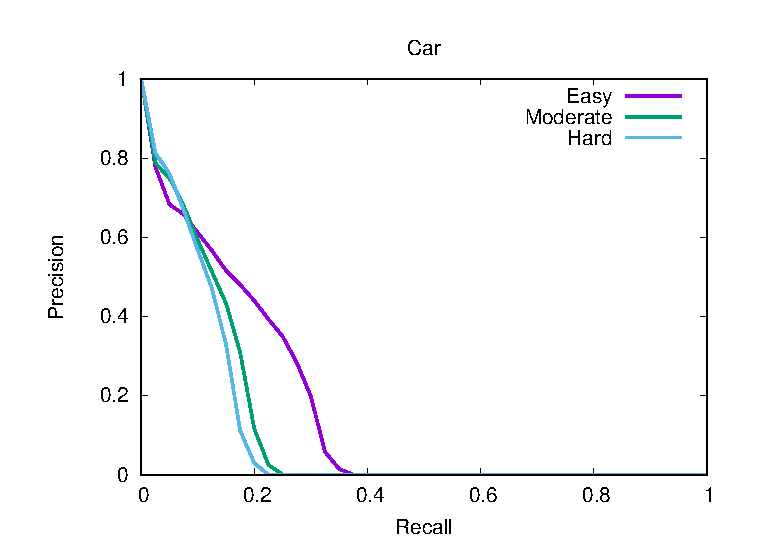
\includegraphics[width=1.0\linewidth]{img/yolo_Nov_4/plot_valid/car_detection.eps}
    \caption{Pre-Trained Yolo on Whole Set}
\end{subfigure}
\begin{subfigure}[t]{.24\textwidth}
    \centering
    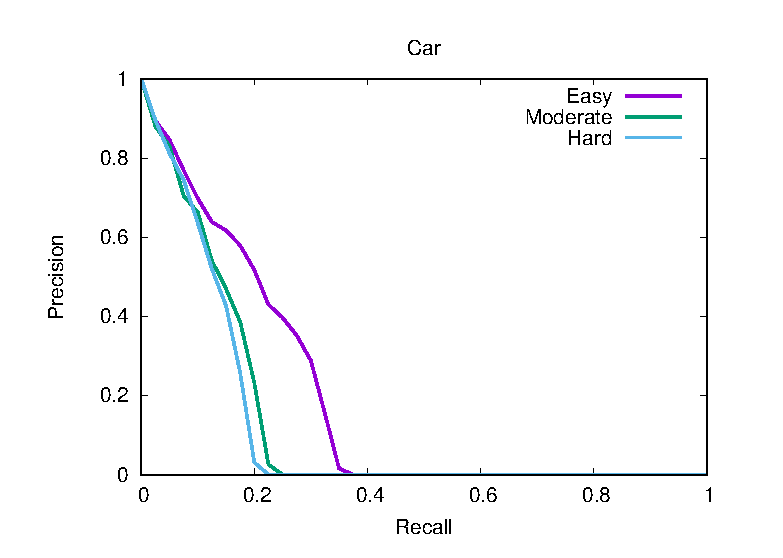
\includegraphics[width=1.0\linewidth]{img/yolo_Nov_4/plot_valid_30/car_detection.eps}
    \caption{Pre-Trained Yolo on Subset}
\end{subfigure}
\begin{subfigure}[t]{.24\textwidth}
    \centering
    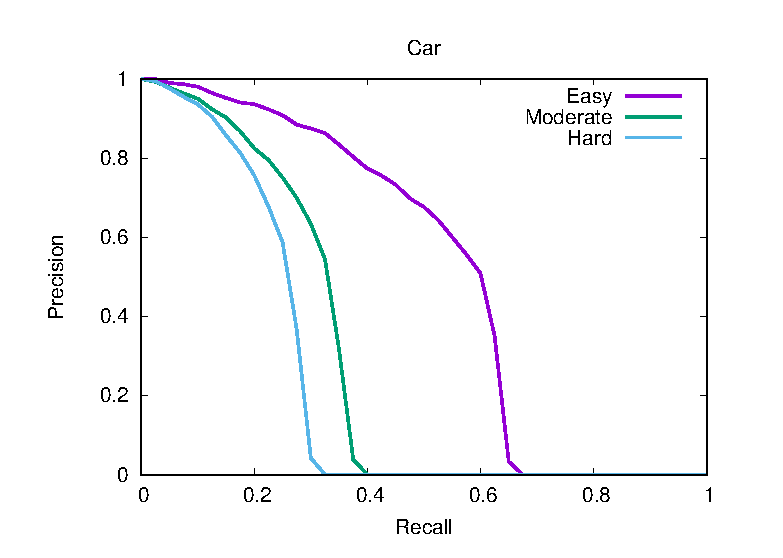
\includegraphics[width=1.0\linewidth]{img/FRCNN_Nov_8/plot_valid/car_detection.eps}
    \caption{Pre-Trained Faster-RCNN on Whole Set}
\end{subfigure}
\begin{subfigure}[t]{.24\textwidth}
    \centering
    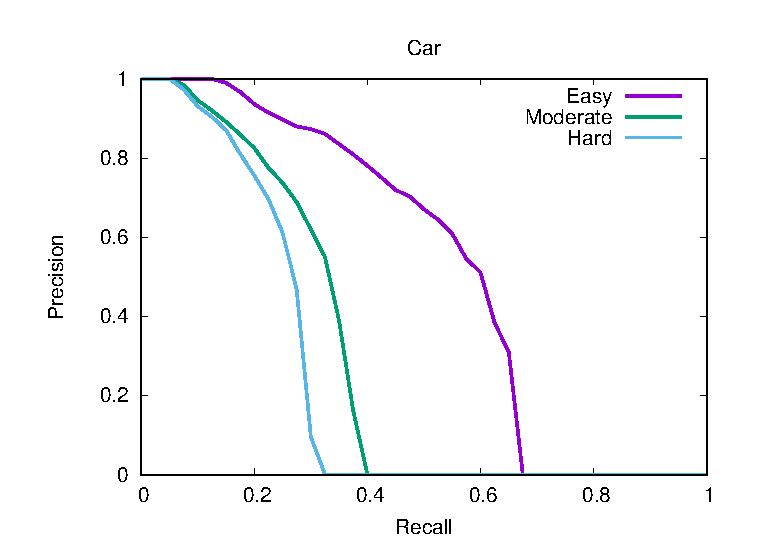
\includegraphics[width=1.0\linewidth]{img/FRCNN_Nov_8/plot_valid_30/car_detection.eps}
    \caption{Pre-Trained Faster-RCNN on Subset}
\end{subfigure}
\caption{Car Detection}
\end{figure}

\begin{table}[h!]
\centering
\begin{tabular}{ c | c | c | c }
\hline
Method & Easy & Moderate & Hard \\
\hline \hline
Pre-Trained Yolo Whole Set & 0.204438 & 0.155358 & 0.145101 \\
Pre-Trained Yolo Subet & 0.227639 & 0.172312 & 0.151478 \\
Pre-Trained Faster-RCNN Whole Set & 0.522754 & 0.309875 & 0.248554 \\
Pre-Trained Faster-RCNN Subet & 0.524807 & 0.308296 & 0.252989 \\
\hline
\end{tabular}
\caption{Average Precision on Car Detection}
\end{table}


\begin{figure}[H]
\centering
\begin{subfigure}[t]{.24\textwidth}
    \centering
    \includegraphics[width=1.0\linewidth]{img/yolo_Nov_4/plot_valid/pedestrian_detection.eps}
    \caption{Pre-Trained Yolo on Whole Set}
\end{subfigure}
\begin{subfigure}[t]{.24\textwidth}
    \centering
    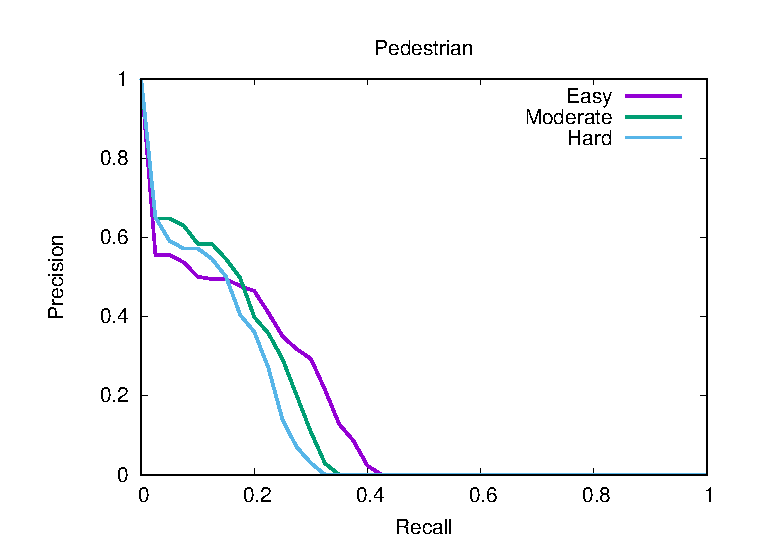
\includegraphics[width=1.0\linewidth]{img/yolo_Nov_4/plot_valid_30/pedestrian_detection.eps}
    \caption{Pre-Trained Yolo on Subset}
\end{subfigure}
\begin{subfigure}[t]{.24\textwidth}
    \centering
    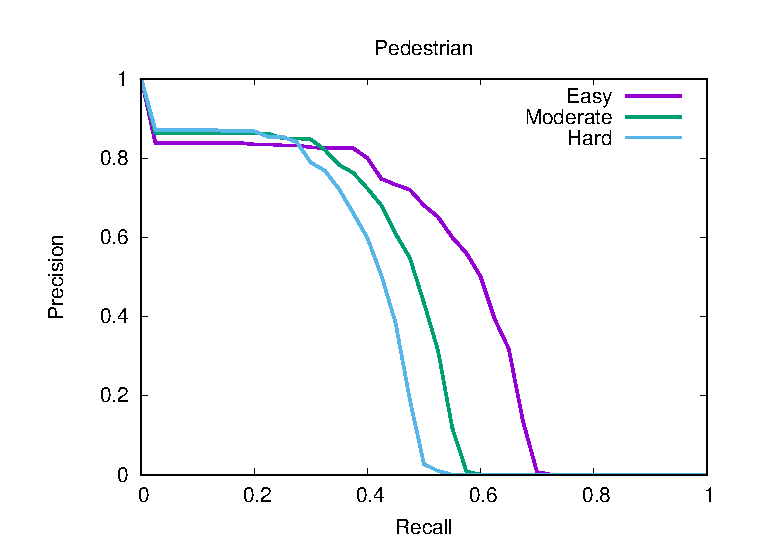
\includegraphics[width=1.0\linewidth]{img/FRCNN_Nov_8/plot_valid/pedestrian_detection.eps}
    \caption{Pre-Trained Faster-RCNN on Whole Set}
\end{subfigure}
\begin{subfigure}[t]{.24\textwidth}
    \centering
    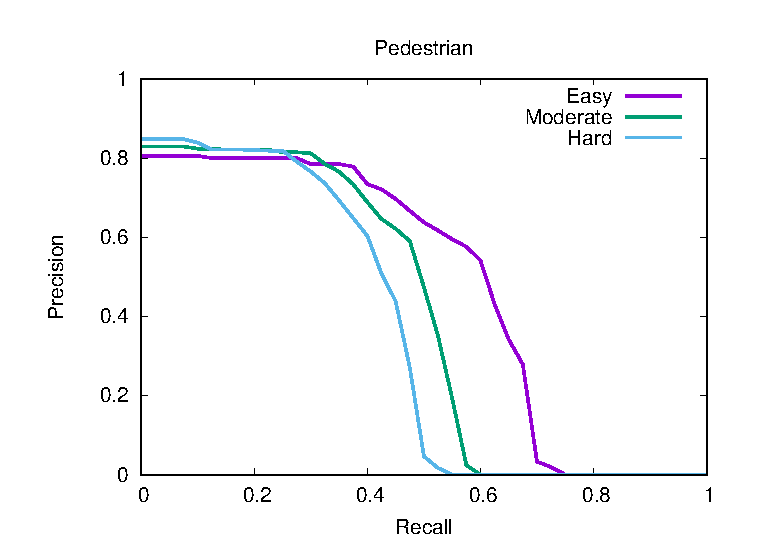
\includegraphics[width=1.0\linewidth]{img/FRCNN_Nov_8/plot_valid_30/pedestrian_detection.eps}
    \caption{Pre-Trained Faster-RCNN on Subset}
\end{subfigure}
\caption{Pedestrian Detection}
\end{figure}

\begin{table}[h!]
\centering
\begin{tabular}{ c | c | c | c }
\hline
Method & Easy & Moderate & Hard \\
\hline \hline
Pre-Trained Yolo Whole Set & 0.197457 & 0.183323 & 0.175022 \\
Pre-Trained Yolo Subet & 0.207263 & 0.189966 & 0.178328 \\
Pre-Trained Faster-RCNN Whole Set & 0.498992 & 0.429862 & 0.377569 \\
Pre-Trained Faster-RCNN Subet & 0.467467 & 0.404372 & 0.356576 \\
\hline
\end{tabular}
\caption{Average Precision on Car Detection}
\end{table}

As we can see, the performance of those two models doesnt' have 
significant difference on the subset compare with the whole set. 
So in all the following experiments, we only work on the subset.

\subsection{Convergence Properties of Different Models}
We build four fine-tuned models, which are
tiny yolo, big yolo, Faster R-CNN using ZFnet and 
Faster-RCNN using VGG\textunderscore CNN\textunderscore M\textunderscore 1024 \cite{chatfield2014return}.

In this section we will show some results about 
their convergence properties by visualizing their loss/error 
changes with iterations.

\begin{figure}[H]
\centering
\begin{subfigure}[t]{.49\textwidth}
    \centering
    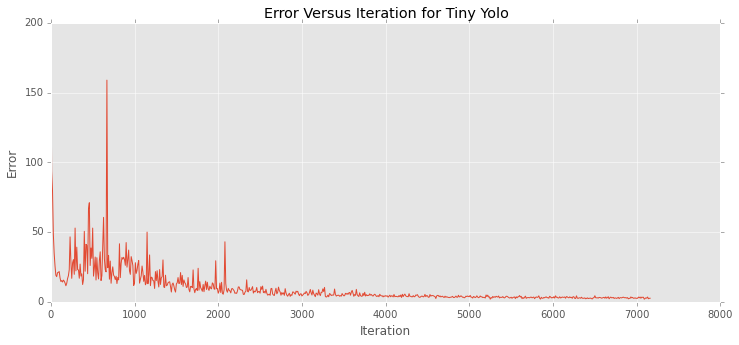
\includegraphics[width=1.0\linewidth]{img/yolo_tiny_cov.png}
    \caption{Tiny Yolo}
\end{subfigure}
\begin{subfigure}[t]{.49\textwidth}
    \centering
    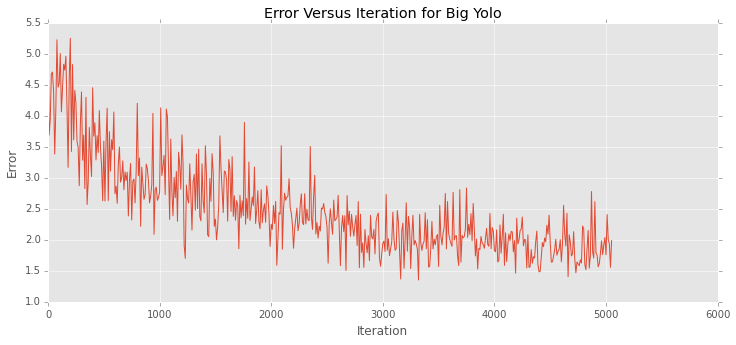
\includegraphics[width=1.0\linewidth]{img/yolo_big_cov.png}
    \caption{Big Yolo}
\end{subfigure}
\caption{Convergence Properties of Yolo}
\end{figure}

\begin{figure}[H]
\centering
\begin{subfigure}[t]{.49\textwidth}
    \centering
    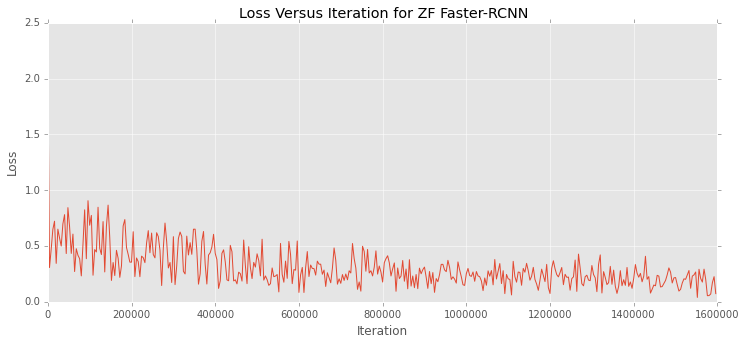
\includegraphics[width=1.0\linewidth]{img/FRCNN_zf_cov.png}
    \caption{Faster R-CNN using ZFnet for Feature Map}
\end{subfigure}
\begin{subfigure}[t]{.49\textwidth}
    \centering
    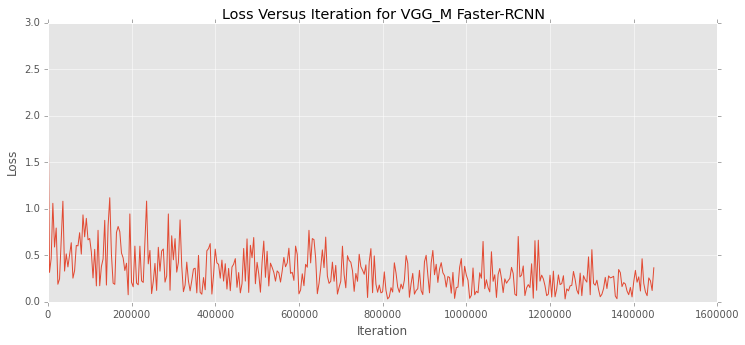
\includegraphics[width=1.0\linewidth]{img/FRCNN_vgg_m_cov.png}
    \caption{Faster R-CNN using VGG\textunderscore CNN\textunderscore M\textunderscore 1024 for Feature Map}
\end{subfigure}
\caption{Convergence Properties of Faster R-CNN}
\end{figure}

As we can see, all the models are very hard to converge even 
with their carefully designed adapting learning rates. 


\subsection{Fine-Tuned Models with Different Network Structure}
In this experiments, we test four different models which has 
different network structure.
A tiny yolo model is a simplified version of the big yolo model 
by reducing 16 convolutional layers for generating features. 
And the difference between two Faster R-CNN models
is using which convolutional networks for generating feature map,
one is ZFnet \cite{zeiler2014visualizing} and the other one is VGG\textunderscore CNN\textunderscore M\textunderscore 1024 \cite{chatfield2014return}. These two convolutional networks 
are quite similar and the main difference is that 
VGG\textunderscore CNN\textunderscore M\textunderscore 1024 
is wider than ZFnet.

We use convolutional weights that are pre-trained on ImageNet classification task as initial weights. Fine tuning models make it possible to benefit from the features the model has learnt previously and speed up training. 

It took about 5 hours to train a tiny yolo after 5,000 iterations
and 15 hours to train a big yolo after 5,000 iterations.
For Faster R-CNN, the one using ZFnet took about 16 hours after 
80,000 iterations and the one using VGG\textunderscore CNN\textunderscore M\textunderscore 1024
took about 12 hours after 80,000 iterations.



\begin{figure}[h!]
\centering
\begin{subfigure}[t]{.32\textwidth}
    \centering
    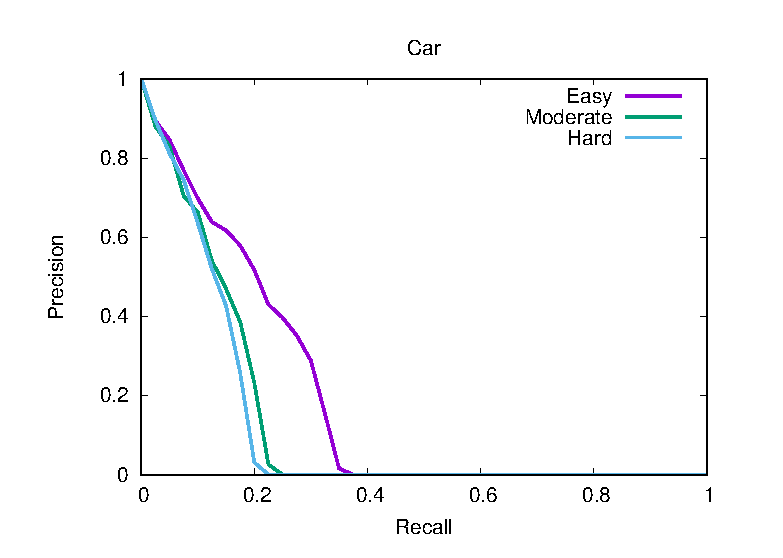
\includegraphics[width=1.0\linewidth]{img/yolo_Nov_4/plot_valid_30/car_detection.eps}
    \caption{Pre-Trained Yolo}
\end{subfigure}%
\begin{subfigure}[t]{.32\textwidth}
    \centering
    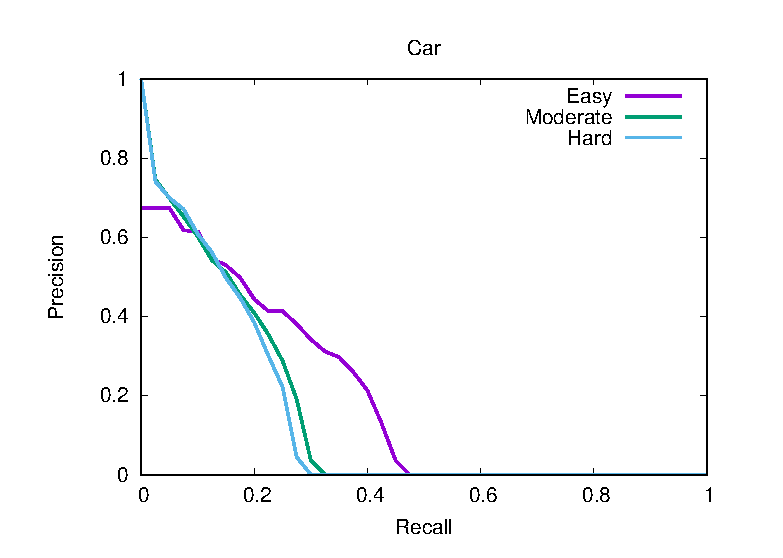
\includegraphics[width=1.0\linewidth]{img/yolo_Dec_7_tiny/plot_valid_30/car_detection.eps}
    \caption{Fine-Tuned Tiny Yolo}
\end{subfigure}%
\begin{subfigure}[t]{.32\textwidth}
    \centering
    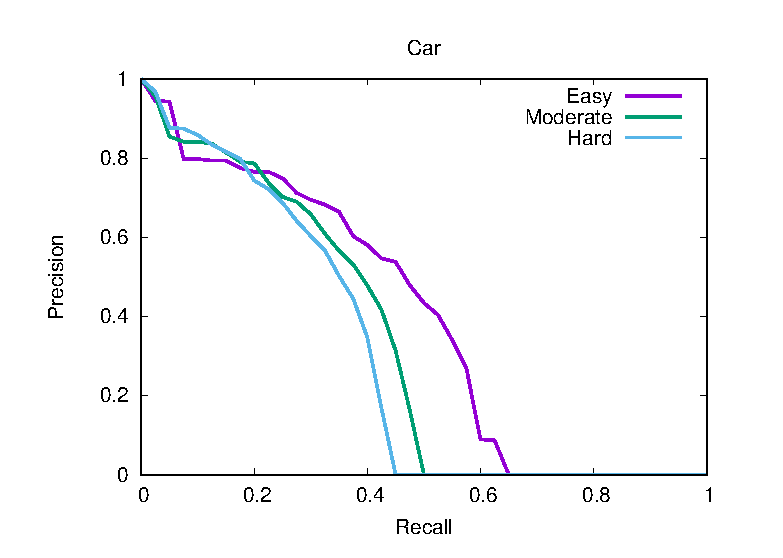
\includegraphics[width=1.0\linewidth]{img/yolo_Dec_7_big/plot_valid_30/car_detection.eps}
    \caption{Fine-Tuned Big Yolo}
\end{subfigure}
\begin{subfigure}[t]{.32\textwidth}
    \centering
    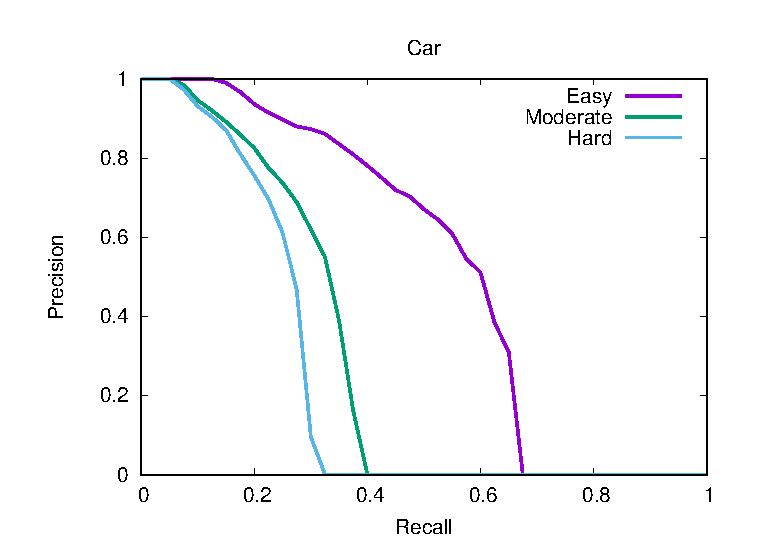
\includegraphics[width=1.0\linewidth]{img/FRCNN_Nov_8/plot_valid_30/car_detection.eps}
    \caption{Pre-Trained Faster R-CNN}
\end{subfigure}%
\begin{subfigure}[t]{.32\textwidth}
    \centering
    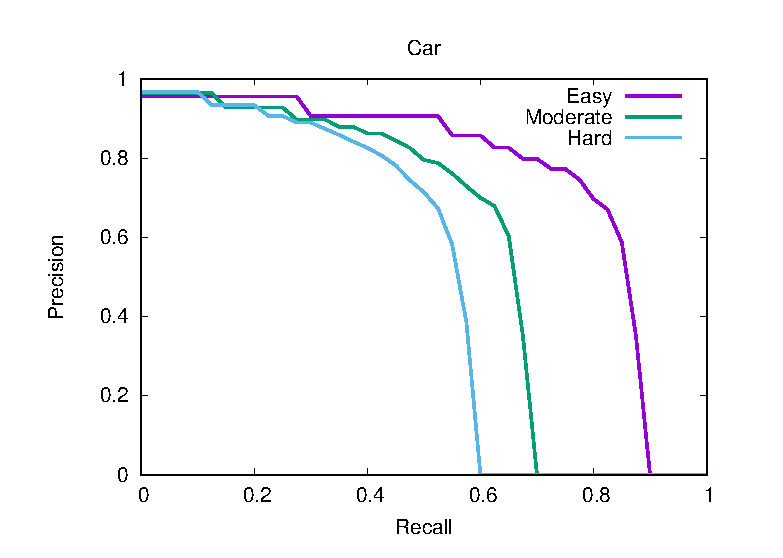
\includegraphics[width=1.0\linewidth]{img/FRCNN_Dec_7_tiny/plot_valid_30/car_detection.eps}
    \caption{Fine-Tuned Faster R-CNN using ZFnet}
\end{subfigure}%
\begin{subfigure}[t]{.32\textwidth}
    \centering
    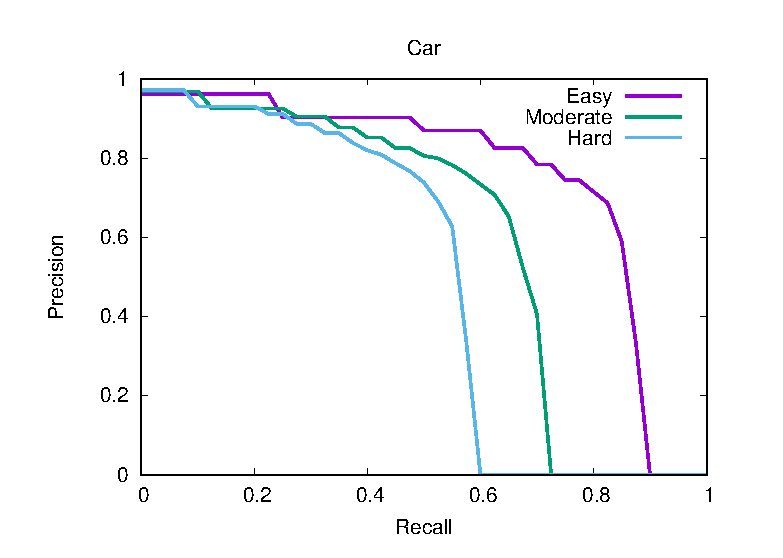
\includegraphics[width=1.0\linewidth]{img/FRCNN_Dec_7_mid/plot_valid_30/car_detection.eps}
    \caption{Fine-Tuned Faster R-CNN using VGG\textunderscore CNN\textunderscore M\textunderscore 1024 }
\end{subfigure}
\caption{Car Detection}
\end{figure}

\begin{table}[h!]
\centering
\begin{tabular}{ c | c | c | c }
\hline
Method & Easy & Moderate & Hard \\
\hline \hline
Pre-Trained Yolo & 0.227639 & 0.172312 & 0.151478 \\
Fine-Tuned Tiny Yolo & 0.207844 & 0.186021 & 0.181117 \\
Fine-Tuned Big Yolo & 0.396407 & 0.342113 & 0.322760 \\
Pre-Trained Faster R-CNN & 0.524807 & 0.308296 & 0.252989 \\
Fine-Tuned ZF Yolo & \bfseries 0.721690 & 0.555533 & \bfseries 0.481580 \\
Find-Tuned VGG\textunderscore M Yolo & 0.721039 & \bfseries 0.596753 & 0.479783 \\
\hline
\end{tabular}
\caption{Average Precision on Car Detection}
\end{table}

\begin{figure}[H]
\centering
\begin{subfigure}[t]{.32\textwidth}
    \centering
    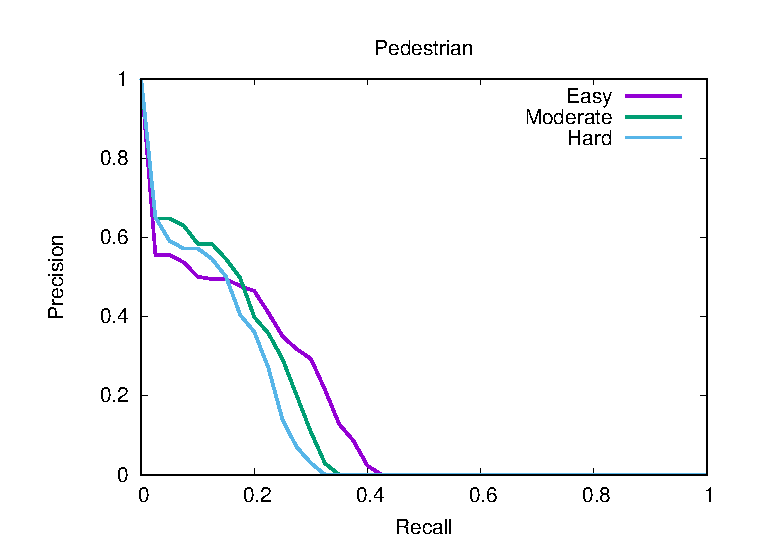
\includegraphics[width=1.0\linewidth]{img/yolo_Nov_4/plot_valid_30/pedestrian_detection.eps}
    \caption{Pre-Trained Yolo}
\end{subfigure}%
\begin{subfigure}[t]{.32\textwidth}
    \centering
    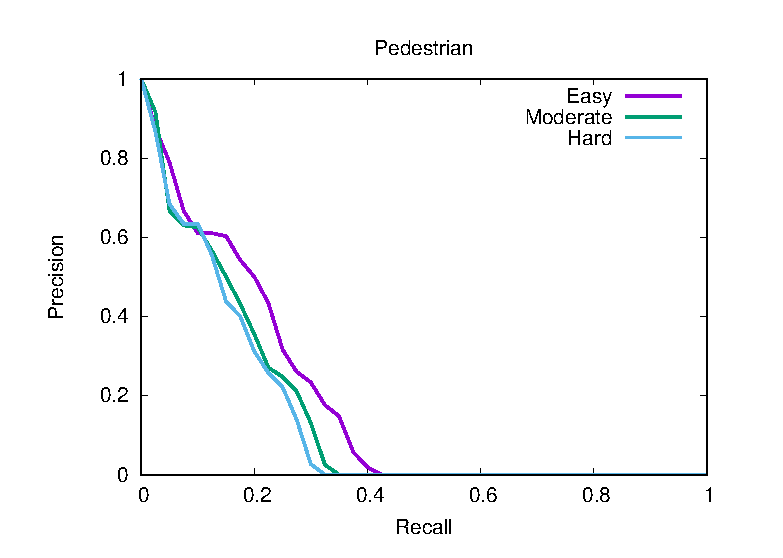
\includegraphics[width=1.0\linewidth]{img/yolo_Dec_7_tiny/plot_valid_30/pedestrian_detection.eps}
    \caption{Fine-Tuned Tiny Yolo}
\end{subfigure}%
\begin{subfigure}[t]{.32\textwidth}
    \centering
    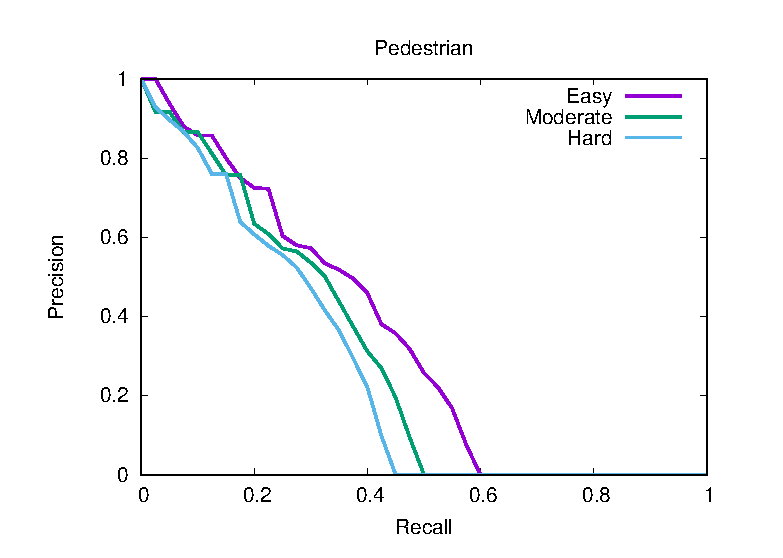
\includegraphics[width=1.0\linewidth]{img/yolo_Dec_7_big/plot_valid_30/pedestrian_detection.eps}
    \caption{Fine-Tuned Big Yolo}
\end{subfigure}
\begin{subfigure}[t]{.32\textwidth}
    \centering
    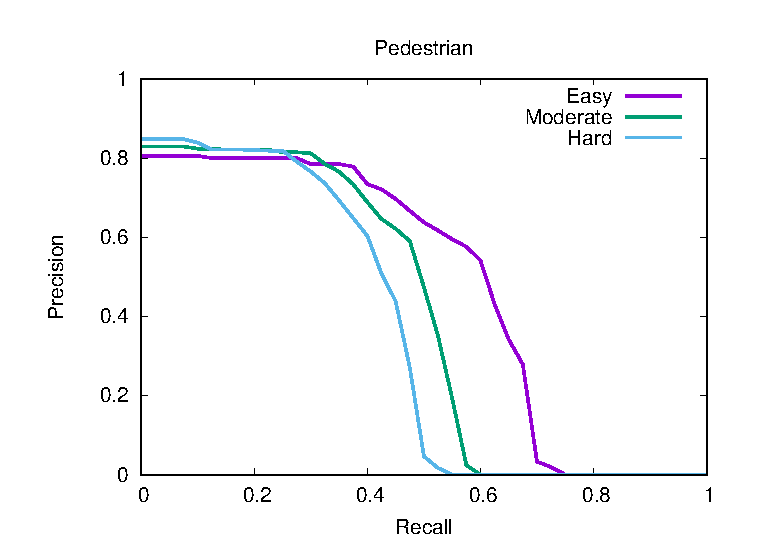
\includegraphics[width=1.0\linewidth]{img/FRCNN_Nov_8/plot_valid_30/pedestrian_detection.eps}
    \caption{Pre-Trained Faster R-CNN}
\end{subfigure}%
\begin{subfigure}[t]{.32\textwidth}
    \centering
    \includegraphics[width=1.0\linewidth]{img/FRCNN_Dec_7_tiny/plot_valid_30/pedestrian_detection.eps}
    \caption{Fine-Tuned Faster R-CNN using ZFnet}
\end{subfigure}%
\begin{subfigure}[t]{.32\textwidth}
    \centering
    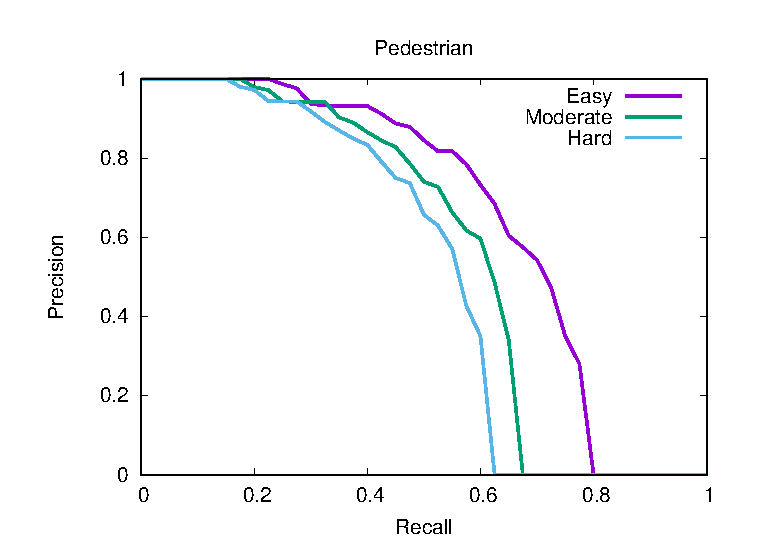
\includegraphics[width=1.0\linewidth]{img/FRCNN_Dec_7_mid/plot_valid_30/pedestrian_detection.eps}
    \caption{Fine-Tuned Faster R-CNN using VGG\textunderscore CNN\textunderscore M\textunderscore 1024 }
\end{subfigure}
\caption{Pedestrian Detection}
\end{figure}

\begin{table}[h!]
\centering
\begin{tabular}{ c | c | c | c }
\hline
Method & Easy & Moderate & Hard \\
\hline \hline
Pre-Trained Yolo & 0.207263 & 0.189966 & 0.178328 \\
Fine-Tuned Tiny Yolo & 0.214768 & 0.191912 & 0.179325 \\
Fine-Tuned Big Yolo & 0.351823 & 0.304227 & 0.284068 \\
Pre-Trained Faster R-CNN & 0.467467 & 0.404372 & 0.356576 \\
Fine-Tuned ZF Yolo &  0.621262 & 0.556017 & \bfseries 0.526138 \\
Find-Tuned VGG\textunderscore M Yolo & \bfseries 0.635249 & \bfseries 0.556700 & 0.520960 \\
\hline
\end{tabular}
\caption{Average Precision on Pedestrian Detection}
\end{table}

\subsection{Detected Object Bounding Boxes}
In this section, we explore the detected object bounding boxes by different 
models by checking the average height, width and area of detected objects. For all the models, we only consider the detected 
object with confidence heigher than 0.2.

\begin{table}[H]
\centering
\begin{tabular}{ c | c | c | c | c}
\hline
Method & Avg Height & Avg Width & Avg Area & cnt \\
\hline \hline
\bfseries Ground Truth & \bfseries 66.6599 & \bfseries 113.2698 & \bfseries 11449.9983 & \bfseries 3188 \\
Fine-Tuned Tiny Yolo & 81.4113 & 130.9231 & 14518.8764 & 2601 \\
Fine-Tuned Big Yolo & 67.6324 & 117.1498 & 11676.8592 & 3029 \\
Fine-Tuned ZF Faster R-CNN & 63.7740 & 102.8394 & 10458.8683 & 3502 \\
Find-Tuned VGG\textunderscore M Yolo & 62.7834 & 100.1970 & 9768.3991 & 3885 \\
\hline
\end{tabular}
\caption{Detected Car Bounding Boxes Comparison}
\end{table}

\begin{table}[H]
\centering
\begin{tabular}{ c | c | c | c | c}
\hline
Method & Avg Height & Avg Width & Avg Area & cnt \\
\hline \hline
\bfseries Ground Truth & \bfseries 103.2774 & \bfseries 43.3553 & \bfseries 6081.0395 & \bfseries 549 \\
Fine-Tuned Tiny Yolo & 158.6333 & 69.7682 & 12327.1655 & 235 \\
Fine-Tuned Big Yolo & 132.4591 & 64.1588 & 9822.6585 & 225 \\
Fine-Tuned ZF Faster R-CNN & 105.9067 & 45.7684 & 6179.3364 & 585 \\
Find-Tuned VGG\textunderscore M Yolo & 96.6618 & 44.1266 & 5529.7738 & 662 \\
\hline
\end{tabular}
\caption{Detected Precision Bounding Boxes Comparison}
\end{table}




